\section{Durchführung und Auswertung}

Bevor wir das SQUID eingeschaltet haben, haben wir die Distanz der Probe zum SQUID-Sensor gemessen. Diese beträgt:

$$z = (3,6 \pm 0,2)\ cm$$

Nach dieser Messung haben wir den flüssigen Stickstoff in das Kryostat gefüllt und den SQUID-Sensor eingefügt. Wir haben 15 Minuten gewartet, und dann mit der Justierung begonnen.

\subsection{Justierung des SQUIDs}

Die Justierung des SQUIDs haben wir anhand des Programms \emph{JSQ Duo Sensor Control} an einem PC und einem Oszilloskop durchgeführt. Wir haben die Software in den Test-Modus geschaltet, welcher einen Funktionsgenerator dazu veranlasst, eine Dreieckspannung in den Schwingkreis einzukoppeln. Diese beeinflusst dann die Spannungsantwort des SQUID, die wir am Oszilloskop einsehen können, das sogenannte \emph{SQUID-Pattern}. Zum Triggern schließen wir dann den Funktionsgenerator noch direkt an den Oszilloskop.  Dann haben wir den Arbeitspunkt anhand der Software justiert, sodass die Amplitude des SQUID-Patterns maximal wurde. Unsere Einstellparameter lauten:\\

\begin{center}
\begin{tabular}[H]{l l}
	$VCA = 1391$ & Stromamplitude des Schwingkreises ($\sim 6\cdot 10^{-8} W$)\\
	$VCO = 1477$ & Frequenz des Schwingkreises ($\sim 760 MHz$)\\
	$OFF = 1471$  & Offset des Signals
\end{tabular}
\end{center}

\begin{figure}[H]
	\centering 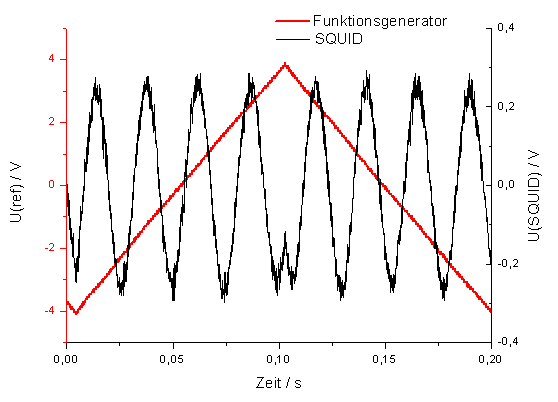
\includegraphics[width = 0.78\textwidth]{Bilder/Pattern1.png}
	\caption{Das SQUID-Pattern}
\end{figure}

\subsection{Dipolmoment und Magnetfeldstärken der Leiterschleife}

\subsubsection{Berechnung}

Wir haben eine stromdurchflossene Leiterschleife mit Durchmesser $d = (3,5 \pm 0,3)\ mm$ am SQUID für 5 verscheide Widerstände gemessen. Aus dem gemessenen Durchmesser ergibt sich der Radius $r=d/2$ mit Fehler $s_r = s_d/2$: $$r = (1,75 \pm 0,15) mm$$

Das magnetische Dipolmoment berechnen wir mit der Formel:

$$p = I\cdot A = \frac{U}{R}\pi r^2 \text{ \ \ \ mit \ \ \ } s_p = p\sqrt{\frac{s_U^2}{U^2} + \frac{s_R^2}{R^2} + 4\frac{s_r^2}{r^2}}$$

Die Feldstärke berechnen wir mit der Formel:

$$B_z = \frac{\mu_0}{2\pi}\frac{p}{z^3} \text{ \ \ \ mit \ \ \ } s_{B_z}=B_z\sqrt{\frac{s_p^2}{p^2} + 9 \frac{s_z^2}{z^2}}$$

Wir erhalten die Werte:

\begin{figure}[H]
	\centering 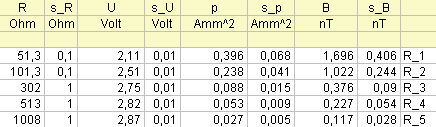
\includegraphics{Bilder/Tab-Leiterschleife.png}
\end{figure}

\subsubsection{Graphisch}

Zur graphischen Berechnung der Dipolmomente und Feldstärken haben wir die Messwerte des SQUIDs sinusförmig gefittet nach der Funktion:

$$ f\left(A,B,C,D,x \right) = A + B\cdot\sin\left(\frac{2 \pi}{180^\circ} C\cdot x + D\right) $$

Hier ist somit A der Offset, B die Amplitude, C die Frequenz und D die Phasenverschiebung. Wir erhalten die Ergebnisse:

\begin{tabular}[H]{| c | c | c | c | c | c |} \hline
 & $\chi^2 / ndf$ & Offset $A$ in $V$ & Amplitude $B$ in $V$ & Frequenz C in $^\circ/s$ & Phase $D$ \\ 
\hline
$R_1$ & 0.82 & -0.6252$\pm$0.0005 & 0.5244$\pm$0.0006 & 49.950$\pm$0.005 & $2.167 \pm 0.002$\\
$R_2$ & 1.64 & 0.6340$\pm$0.0006 & 0.2722$\pm$0.0009 & 49.916$\pm$0.014 & $-2.682 \pm 0.007$\\
$R_3$ & 0.22 & -0.5370$\pm$0.0002 & 0.0916$\pm$0.0003 & 49.936$\pm$0.015 & $3.208 \pm 0.007$\\
$R_4$ & 0.20 & -0.5263$\pm$0.0002 & 0.0546$\pm$0.0003 & 50.048$\pm$0.023 & $0.178 \pm 0.001$\\
$R_5$ & 0.32 & -0.6587$\pm$0.0003 & 0.0247$\pm$0.0004 & 49.953$\pm$0.071 & $3.032 \pm 0.035$\\ \hline
\end{tabular}

Die Graphen, sowie deren Fits und Polarplots kann man im Anhang einsehen.

Mit der Formel 

$$ B_z = F \frac{\Delta V}{2s_i} = F\frac{B}{s_i} $$

berechnen wir anhand der Fits die Feldstärke. Es gilt $\Delta V = 2B$. $F = 9.3 nT / \Phi_0$ ist der Feld-Fluss-Koeffizient, der Wert ist eine Herstellerangabe. $s_i$ ist der eingestellte Wert des Feedback-Resistors und beträgt in allen Fällen $1,9 V/ \Phi_0$. Der Fehler auf $B_z$ berechnet sich durch:

$$ s_{B_z} = B_z\frac{s_B}{B} $$

(B ist hier die aus den Fits bestimmte Amplitude der Sinusfunktion)
 
Die erhaltenen Werte haben wir in einer Tabelle zusammengefasst, um den direkten Vergleich mit den berechneten Werten zu erleichtern:

\begin{center}
\begin{tabular}[H]{| c | c | c |} \hline
 & $B_z / nT$ berechnet & $B_z / nT$ aus dem Fit\\ \hline \hline
 $R_1$ & $1,696 \pm 0,219$ & $2,567\pm 0,003$\\
 $R_2$ & $1,022 \pm 0,132$ & $1,333\pm 0,004$\\
 $R_3$ & $0,376 \pm 0,048$ & $0,448\pm 0,001$\\
 $R_4$ & $0,227 \pm 0,029$ & $0,267\pm 0,001$\\
 $R_5$ & $0,117 \pm 0,015$ & $0,121\pm 0,002$\\ \hline
 \end{tabular}
 \end{center}
 
 Wie man gut erkennen kann, ist vor allem die Abweichung der Werte für $R_1$ sehr groß. Die anderen Werte liegen alle mehr oder weniger im tolerierbaren Bereich aneinander.
 
 Aus der magnetischen Feldstärke können wir das magnetische Dipolmoment der Leiterschleife für die einzelnen Widerstände mit folgender Formel berechnen:
 
$$ B_z = \frac{\mu_0}{2\pi}\frac{p}{z^3} \ \Leftrightarrow \  p = \frac{2\pi z^3}{\mu_0}B_z $$

mit dem Fehler:

$$s_p = p\sqrt{\frac{s_{B_z}^2}{B_z^2} + 9\frac{s_z^2}{z^2}}$$

Wir erhalten die Werte (im Vergleich mit den Berechneten):

\begin{center}
\begin{tabular}[H]{| c | c | c |} \hline
 & $p$ in $A\cdot mm^2$ berechnet & $p$ in $A\cdot mm^2$ aus dem Fit\\ \hline \hline
 $R_1$ & $0,369 \pm 0,068$ & $0,599\pm 0,100$\\
 $R_2$ & $0,283 \pm 0,041$ & $0,311\pm 0,052$\\
 $R_3$ & $0,088 \pm 0,015$ & $0,105\pm 0,017$\\
 $R_4$ & $0,053 \pm 0,009$ & $0,062\pm 0,010$\\
 $R_5$ & $0,027 \pm 0,005$ & $0,028\pm 0,005$\\ \hline
 \end{tabular}
 \end{center}
 
 Auch hier kann man gut erkennen, dass vor allem die Werte für $R_1$ stark voneinander abweichen.

\subsection{Dipolmoment und Feldstärke anderer Proben}

Nach der Leiterschleife, haben wir andere Proben in das SQUID eingeführt und vermessen. Die Auswertung haben wir wieder mit der Sinus-Funktion $f(x) = A + B\sin(Cx+D)$ gemacht. Hier eine Tabelle der Proben und deren Fit-Werte.

\begin{center}
\begin{tabular}[H]{| l | c | c | c | c |} \hline 
 & $\chi^2 / ndf$ & Offset $A$ in $V$ & Amplitude $B$ in $V$ & Frequenz C in $^\circ/s$\\ 
\hline \hline
{Metallbolzen} & 303 & -2.7585$\pm$0.0087 & 7.1330$\pm$0.0123 &	 49.7482$\pm$0.0070\\
{Magnetspan $\perp$} & 267 & -7.6301$\pm$0.0082 & 5.6332$\pm$0.0116 & 49.7893$\pm$0.0081\\
{Magnetspan 45$^\circ$} & 706 & -5.3528$\pm$0.0133 & 8.6427$\pm$0.0187 & 49.7974$\pm$0.0087\\
{Magnetspan //} & 344 & -5.8435$\pm$0.0093 & 7.8321$\pm$0.0132 & 49.7035$\pm$0.0066\\
{Steinzylinder} & 0.33 & 0.04678$\pm$0.0003 & -0.0043$\pm$0.0004 & 44.0235$\pm$0.4014\\
{Eisenspan //} & 0.05 & -0.0101$\pm$0.0001 & 0.0122$\pm$0.0001 & 49.7288$\pm$0.05103\\
{Eisenspan$\perp$} & 0.04 & 0.0074$\pm$0.0001 & -0.0126$\pm$0.0001 & 49.6935$\pm$0.0438\\
{Gold} & 0.002 & 0.0012$\pm$0.0001 & 0.0001$\pm$0.0001 & 21.6771$\pm$2.0544\\ %Gold1
{Heller Stein} & 0.18 & 0.0183$\pm$0.0002 & 0.0024$\pm$0.0003 & 47.0429$\pm$0.3391\\
{ISE Zugangsschlüssel} & 0.02 & 0.0024$\pm$0.0001 & 0.0001$\pm$0.0001 & 24.8102$\pm$2.9728\\
{Kronkorken} & 237 & -1.6482$\pm$0.0077 & 3.5751$\pm$0.0109 & 49.8015$\pm$0.0122\\ %1
{Kaffeeschlüssel} & 4.42 & 0.0083$\pm$0.0011 & 0.1781$\pm$0.0015 & 49.8351$\pm$0.03293\\
{iPod Shuffle} & 8173 & -4.3923$\pm$0.0453 & 4.6443$\pm$0.0638 & 49.8386$\pm$0.0555\\
\hline
\end{tabular}
\end{center}

Die Suffixe // (parallel), $\perp$ (senkrecht) und \emph{45$^\circ$} bezeichnen hier die Ausrichtung der Probe zum Stab des Motors. Wie man erkennen kann entsprechen die Frequenzen für das Gold und den ISE-Zugangsschlüssel nicht dem Wert der anderen Frequenzen (obwohl der Motor immer gleich eingestellt war). Dies deutet daraufhin, dass diese Proben keine mit dem SQUID messbaren Dipolmomente haben. Wie man an den Graphen im Anhang erkennen kann, sind diese Verläufe auch nicht wirklich sinusförmig so dass der Fit nicht wirklich angebracht ist. Trotzdem haben wir diese pro forma ausgewertet und das Dipolmoment und die magnetische Feldstärke berechnet.

Wichtig ist hier zu bemerken, dass wir nach der Messung des Goldes flüssiges Stickstoff in das SQUID nachgefüllt haben. Wir mussten danach also nochmal das SQUID justieren. Das neu eingestellten Parameter lauten

\begin{center}
\begin{tabular}[H]{l l}
	$VCA = 1441$ & Stromamplitude des Schwingkreises ($\sim 6\cdot 10^{-8} W$)\\
	$VCO = 1477$ & Frequenz des Schwingkreises ($\sim 760 MHz$)\\
	$OFF = 1446$  & Offset des Signals
\end{tabular}
\end{center}

und das Pattern sieht folgendermaßen aus:

\begin{figure}[H]
	\centering 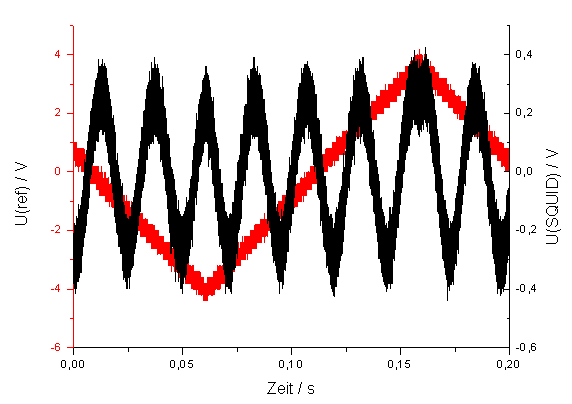
\includegraphics[width = 0.8\textwidth]{Bilder/Pattern2.png}
	\caption{Das zweite SQUID-Pattern}
\end{figure}


Zur Auswertung der obigen Tabelle benutzen wir (wieder) folgende Formeln;

$$ B_z = F\frac{B}{s_i} \text{ \ \ , \ \ } s_{B_z} = B_z\frac{s_B}{B}$$

$$ p = \frac{2\pi z^3}{\mu_0}B_z \text{ \ \ , \ \ } s_p = p\sqrt{\frac{s_{B_z}^2}{B_z^2} + 9\frac{s_z^2}{z^2}} $$

Wir erhalten:

\begin{figure}[H]
	\centering 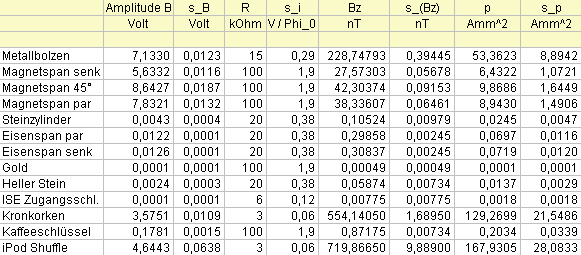
\includegraphics[width=\textwidth]{Bilder/Tab-Proben.png}
\end{figure}

Wie man sieht sind die Feldstärken/Dipolmomente beim Metallbolzen, Kronkorken und iPod Shuffle (ausgeschaltet!) am höchsten. Der Magnetspan hat auch ein relativ starkes Dipolmoment/Feld. Das Gold und der ISE-Zugangsschlüssel haben wie erwartet kaum ein Dipolmoment (Feldstärke), bzw. ein vernachlässigbares, da der Fehler hier so groß wie der Wert selber ist. Die Werte vom Steinzylinder und dem Eisenspan sind vergleichbar mit den Werten der Leiterschleife ($R_3$ bis $R_5$). Der helle Kieselstein hat auch kaum ein Dipolmoment/eine Feldstärke, der Kaffeeschlüssel hingegen ist wiederum im Bereich der Leiterschleife bei $R_2$.















